\documentclass[crop,tikz]{standalone}

\usepackage{pgfplots}
\pgfplotsset{compat=1.18}

\pgfplotsset{
  inverted/.style = {
    every axis legend/.append style={
      draw=white,
      fill=black,
      text=white
    }
  }
}

\begin{document}
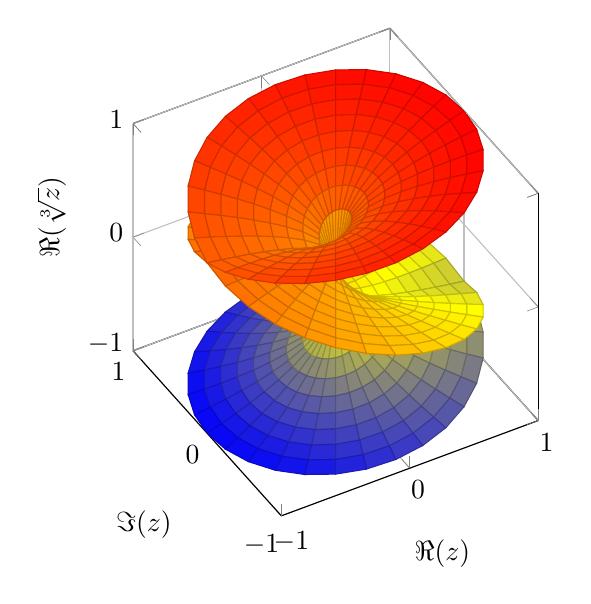
\begin{tikzpicture}
  \begin{axis}[
    width=15cm,
    axis equal image,
    view={-30}{40},
    xlabel={$\Re(z)$},
    ylabel={$\Im(z)$},
    zlabel={$\Re(\sqrt[3]{z})$},
    xmin=-1,xmax=1,
    ymin=-1,ymax=1,
    zmin=-1, zmax=1,
    samples=10, samples y=91,
    domain=0:1, domain y=0:{3*360},
    z buffer=sort,
    grid,
    ]
    \addplot3[surf,colormap/hot] ({x*cos(y)},{x*sin(y)},{x^(1/3)*cos(y/3)});
  \end{axis}
\end{tikzpicture}
\end{document}
